\section{Hardware für Privatanwender}\label{s:DIY}

In den letzten Jahren sind viele Privatanwender aufgrund der sich bietenden Möglichkeiten dazu übergegangen, eigene Anwendungen mit kleinen \ac{IoT}-Systemen selbst zu entwickeln. Hierzu werden meist kleine Einplatinencomputer verwendet, da diese sehr günstig zu erhalten sind. 
Zwei der erfolgreichsten Einplatinen Computer sind die Modelle der Raspberry Pi und Arduino Familie.


\subsection{Arduino-Plattform}\label{ss:Arduino}

Arduino ist ein Unternehmen, das all seine Produkte in enger Zusammenarbeit mit zugehörigen Community entworfen hat. Alle Entwicklungen basieren auf den Ideen und Konzepten, die die Gemeinschaft um das Unternehmen entwickelt hat. 

\begin{figure}[H] 
	\centering
	
\includegraphics[scale=0.2]{Bilder/arduino}
	\caption{Das Arduino-Logo\cite{i:arduino}}
	\label{f:arduino}
\end{figure}

Das Unternehmen entwickelt Mikrokontrollerplatinen, die ihre Umwelt durch Sensoren wahrnehmen und auf äußere Einflüsse reagieren können. Alle Produkte sind vorgefertigt oder als Selbstbau-Kit erhältlich. Da die Baupläne aller Platinen durch Arduino quelloffen im Internet erhältlich sind, können die Produkte auch von Grund auf nachentworfen werden.\\

Das erste Arduino-Board, dass 2005 vorgestellt wurde, hat bereits viele Revisionen erhalten. In der aktuellsten Version ist es mit einem 16 \ac{MHz} 8-Bit Microcontroller ATmega328 der Firma Atmel bestückt. Es besitzt zusätzlich 32 Kilobyte Flash-Speicher von dem 0.5 Kilobyte durch den Bootloader belegt werden. Zur Ein- und Ausgabe, sowie zum Anschließen von Sensoren besitzt die Platine 14 digitale Input- oder Output-Pins, sowie 6 analoge input Pins und einen \ac{USB}-Anschluss. Betrieben wird die Platine mit einem 7-12V Netzteil \cite{ws:arduinouno}.
Die Platine wird von dem italienischen Unternehmen SmartProjects produziert, ist jedoch aufgrund des quelloffenen Platinenplans auch selbst zusammensetzbar.\\

\begin{figure}[H] 
	\centering
	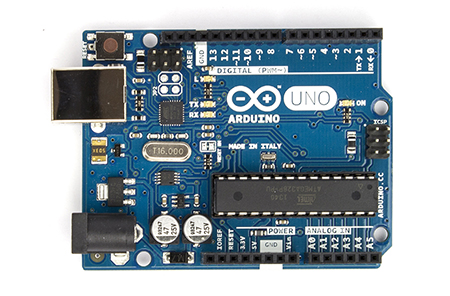
\includegraphics[scale=0.6]{Bilder/arduinouno}
	\caption{Die Front der dritten Arduino Uno Revision\cite{i:arduinouno}}
	\label{f:arduinouno}
\end{figure}

Die Arduino-Plattform besitzt eine eigene \ac{IDE}, in der die Software für den Microcontroller entwickelt werden kann. Der Mikrocontroller wird mit einer stark vereinfachten Form der Programmiersprachen C und C++ angesprochen. Insbesondere technische Informationen wie Header-Files werden vor dem Programmierer verborgen. Für Anfänger bietet die \ac{IDE} mehrere Einstiegshilfen, die das Programmieren erleichtern.\\
Ein Beispiel für die Einstiegshilfen sind die strukturgebenden Funktionen setup(), sowie loop(). Während in der Setup-Methode alle Aktionen definiert werden müssen, die beim Programmstart durchgeführt werden sollen, wird der Code in der Loop-Methode unbegrenzt oft wiederholt.
Ein Beispielcode, der eine an Pin 13 angeschlossene LED blinken lässt, lautet wie folgt:\\

\begin{lstlisting}[language=c,caption={Simpler Arduino-Code, der eine LED blinken lässt},label=lst:blink,frame=single] 
int led = 13; //LED an Pin 13

void setup() {                
	pinMode(led, OUTPUT);     
}

void loop() {
	digitalWrite(led, HIGH);  
	delay(1000);               
	digitalWrite(led, LOW);   
	delay(1000);               
}
\end{lstlisting}

\vspace{1cm}

Seit der Entwicklung der Arduino-Boards erfreuen sich diese großer Beliebtheit. So wurden bis 2013 insgesamt 700.000 zusammengesetzte Platinen verkauft\cite{ws:sellnumb}.\\

Viele der Projekte, die mit Arduino-Platinen durchgeführt werden, beinhalten Benutzerinteraktion. Auch für Kunstinstallationen werden die Einplatinencomputer gerne verwendet\cite{ws:elektor}.

\subsection{Raspberry Pi}\label{ss:Raspberry}

Die in Großbritannien angesiedelte Wohltätigkeitsorganisation "Raspberry Pi Foundation" hat es sich zur Aufgabe gemacht, Einplatinencomputer für Menschen zu entwickeln, die Hardware- oder Programmierkenntnisse erwerben wollen. Um auch für Jugendliche und Studenten ansprechend zu sein, wurde ein besonders geringer Verkaufspreis angestrebt. Die verschiedenen Modelle des Raspberry Pis kosten zwischen 20 und 35 US-\$ und sind somit sehr günstig.\\

Der Name setzt entstand durch die aus der Kombination zweier Gedanken. Viele Computer wurden nach Früchten benannt (z.B. Apple), aus diesem Grund entschieden sich die Gründer für Raspberry. Der Namenszusatz Pi entstand aus dem Ursprünglichen plan, die Raspberry Pi Einplatinencomputer mit einem Phyton Interpreter auszuliefern, daher das die Abkürzung PI. Als Ergebnis eines öffentlich ausgeschrieben Wettbewerbs wurde eine silisierte Himbeere als Logo für die Wohltätigkeitsorganisation gewählt.

\begin{figure}[H] 
	\centering
	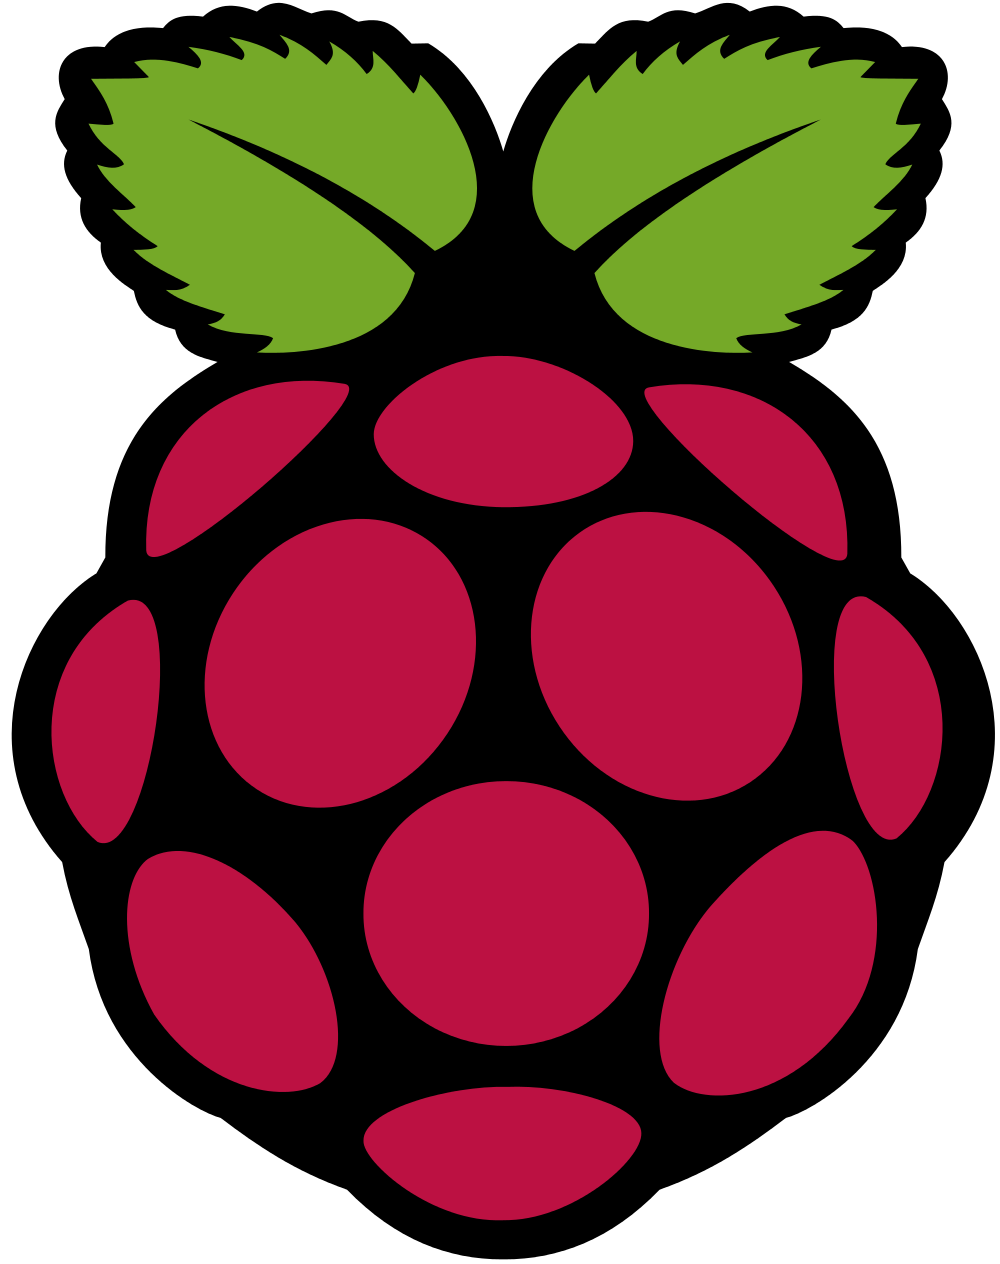
\includegraphics[scale=0.15]{Bilder/raspberrylogo}
	\caption{Das Logo der Raspberry Pi Foundation\cite{i:raspberrylogo}}
	\label{f:raspberrylogo}
\end{figure}

Insgesamt bietet die Raspberry Pi Foundation sechs Modelle des Computers an. Eine sehr grundlegende ausführung, das Compute Module, dass nur in Stückzahlen über 100 verkauft wird, sowie die günstigen Modelle A und A+, die mit 25 und 20 US-\$ am unteren Preisende liegen. Die Modelle B, B+, sowie das überarbeitete Modell Generation 2 B sind am oberne Preisende, mit jeweils 35 US-\$ angesiedelt. \\

\begin{figure}[H] 
	\centering
	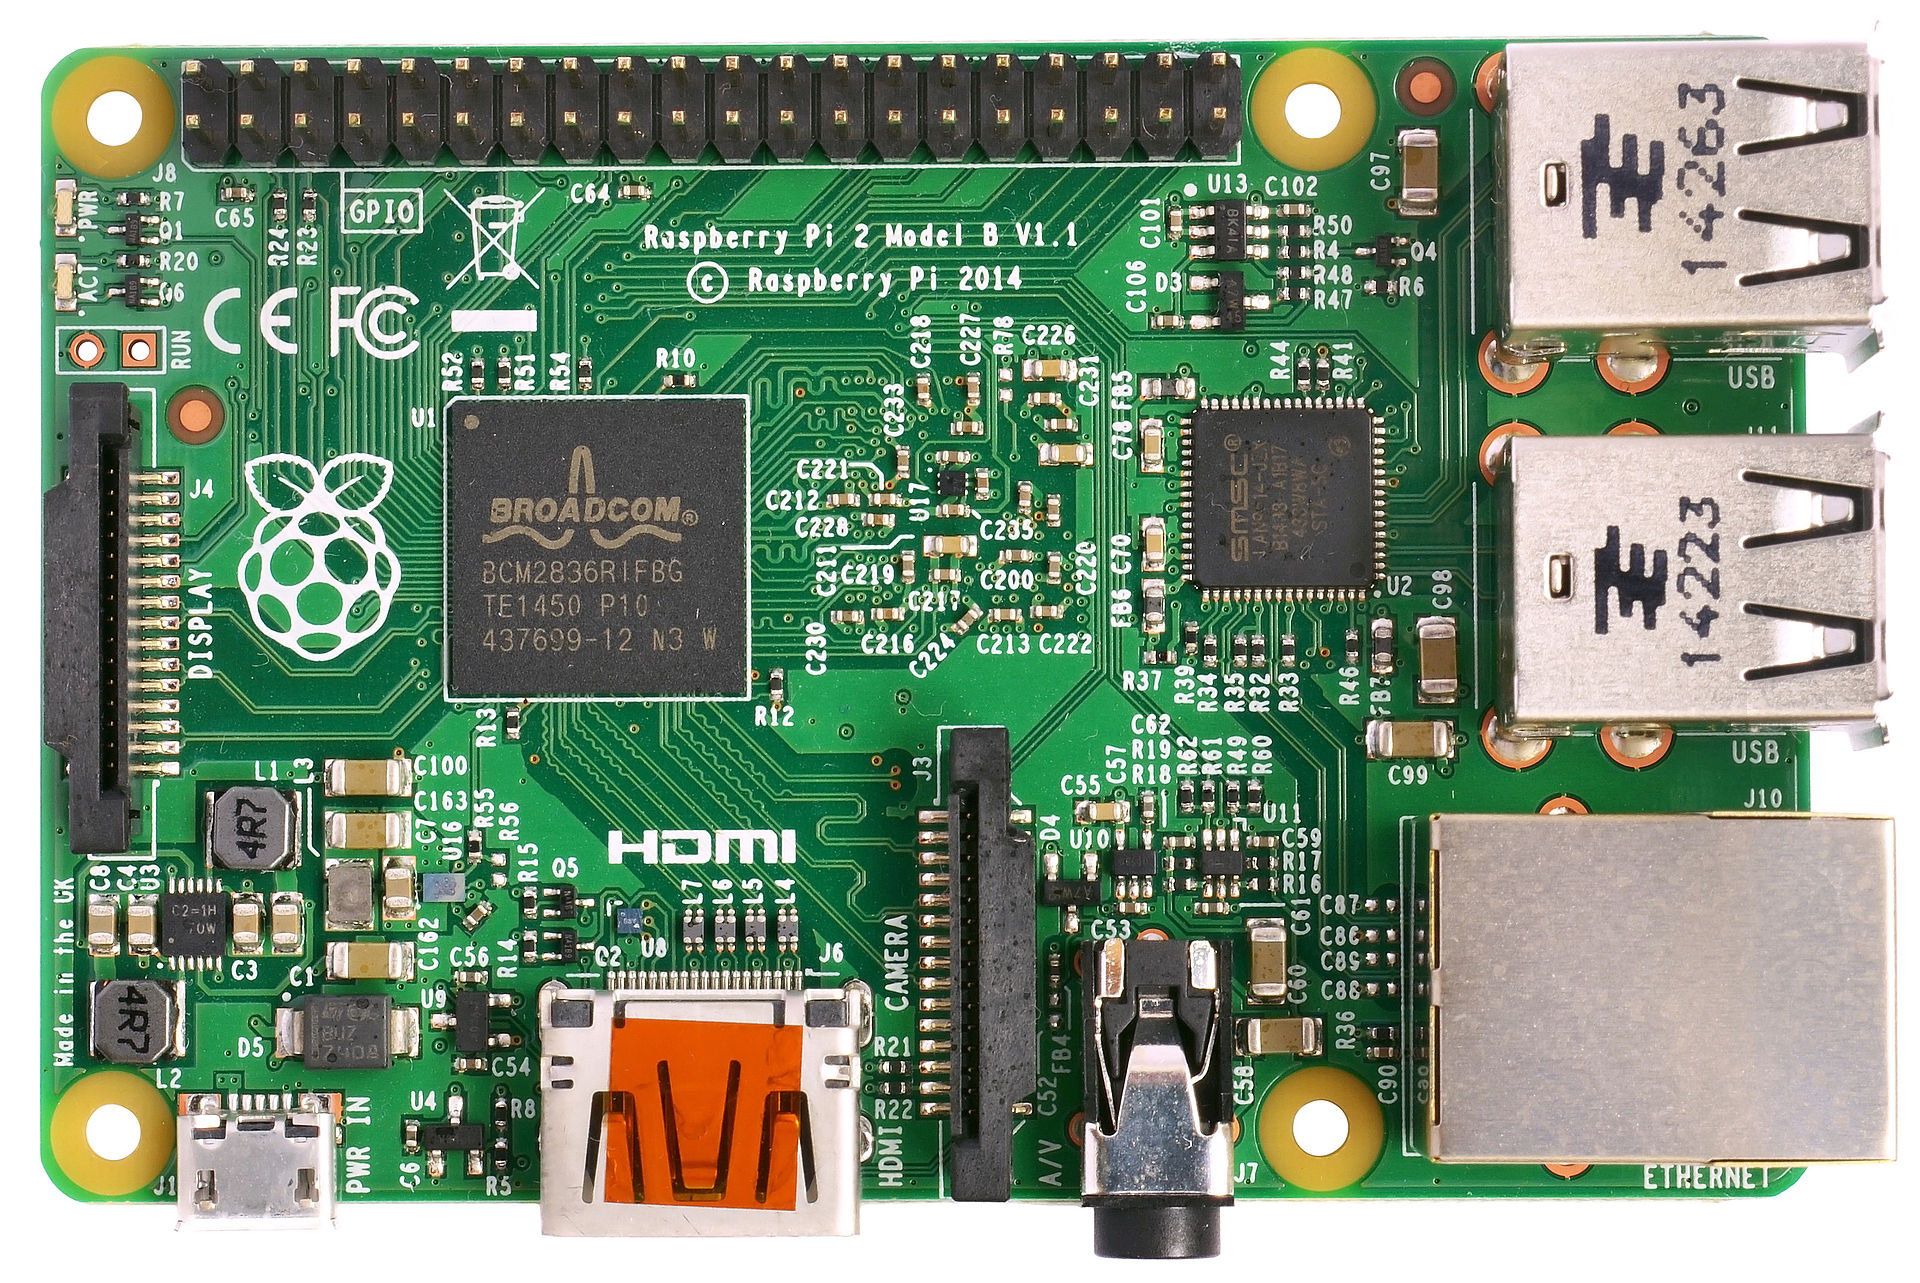
\includegraphics[scale=0.5]{Bilder/raspberry2top}
	\caption{Die Oberseite des Raspberry Generation 2 B-Modells\cite{i:raspberry2top}}
	\label{f:raspberry2top}
\end{figure}

Mit dem Anfang 2015 vorgestellten Generation 2 B - Modell wurde ein Performancesprung realisiert. 
Mit dem System-on-a-Chip Broadcom BCM2836, das sowohl CPU als auch GPU des Einplatinencomputers darstellt sind auf vier Kernen berechnungen mit bis zu 900 \ac{Mhz} möglich. Dies wird mit 1 Gigabyte Arbeitsspeicher zu einem, für den geringen Preis, leistungsstarken System kombiniert.
Die Hardwarekomponenten des Generation 2 B -Modells sind so leistungsstark, dass das ausführen von Windows 10 möglich ist.\\

Auch in Sachen I/O-Anschlüsse ist der Raspberry Pi gut ausgerüstet. Er stellt insgesamt 17 Pins bereit, die sowohl als Input, sowie Output genutzt werden können. Zusätzlich verfügt der Raspberry Pi über 4 \ac{USB}-Ports, einen HDMI-Anschluss und einen MicroSD-Karten Slot. Dieser wird als Speicher für das Betriebssystem und alle Programme verwendet.\\
Um den Raspberry Pi mit Netzwerken zu vebrinden besitzt der Raspberry ein 100Mbit Netzwerkanschluss.

Über Micro-\ac{USB} wird die Platine mit 


